%%=========================================
\section[Teori \& Relatert arbeid]{Teori \& Relatert arbeid}
%%=========================================
\subsection{Smarte hjem}
\label{ch:smartehjem}
I introduksjonen definerte jeg smarte hjem til å være boliger der miljøet og apparater kan programmeres og styres. Dette er ikke ny teknologi. Muligheten for å kontrollere hus og hytter på avstand har vært tilgjengelig for de mest interesserte i lang tid. \citet{peine08} viser til at idéen om smarte hjem har vært beskrevet siden 80-tallet, men har i de senere år fått en ny interesse i industrien. Styring i kontorbygninger har eksistert siden 70-tallet, med muligheter for å kontrollere lys, varme, elektrisitet og adgangskontroll fra et sentralt sted. Det tok noen år før man innså at de samme egenskapene kunne være ønskelige i private hjem. Forskjellen mellom et vanlig hjem og et smart hjem, er altså denne muligheten til å styre flere aspekter ved hjemmet gjennom en sentral enhet.

På markedet finnes det nå flere løsninger for å automatisere deler av hjemmet eller som tilbyr brukergrensesnitt for å styre funksjonalitet som lys og varme. Disse løsningene bidrar med å ivareta sikkerhet og å begrense energiforbruk. Det tilbys gjerne informasjon om hjemmet via en app til smarttelefonen slik at brukeren kan ha oversikten selv når han er bortreist. Ved å installere moderne enheter med internettilknytning, som termostater, lys, låser, \\sikkerhetssystemer og garasjeporter, kan brukeren avlese informasjon og styre enhetene med smarttelefonen.

Denne neste generasjonen apparater med internettilkobling bringer spennende muligheter, men samtidig utfordringer. \emph{Tingenes internett} spås en enorm vekst de neste årene. Se for deg følgende scenario: alle elektriske enheter og apparater, lys, dører, persienner og et stort antall sensorer for å måle temperatur, bevegelse og tilstedeværelse; alle koblet til internettet. Det vil være en utfordring å håndtere alle disse dataene på en ansvarlig måte. Det vil være en utfordring å tilby gode måter for å lære om og styre hjemmet.

Det finnes ikke et eget fagområde for smarte hjem. Teknologiene og teknikkene som kan brukes for å skape smarte hjem har tilknytning til en rekke fagområder, som bygningsautomasjon, robotikk, nettverk, sikkerhet, menneske-maskin-interaksjon (HCI), kunstig intelligens (AI) og ambient intelligens (AmI).

AmI er spesielt interessant i kontekst av smarte hjem fordi det omhandler miljøer som er sensitive og responsive til mennesker. Det er en visjon på hvordan vi bruker teknologi i omgivelsene for å støtte opp under hverdagslige aktiviteter. Ettersom enhetene som utgjør denne teknologien stadig blir mindre, og stadig blir bedre på å kommunisere seg i mellom, vil teknologien forsvinne inn i omgivelsene. Det eneste synlige vil være brukergrensesnittene vi har designet for å aktivt interagere med teknologien. Dette er en videreføring av framtidssynet \citet{weiser91} skriver om, der teknologien forsvinner inn i omgivelsene og hverdagslivet inntil det er umulig å skille de fra hverandre. AmI omhandler alle miljøer vi befinner oss i og omhandler dermed også hjemmet.

For å være til hjelp for oss må hjemmet forstå omgivelsenens tilstand og det vil være nødvendig å analysere sensorinformasjon. Jeg har allerede nevnt enkle sensorer, som temperatur og bevegelse, og i kombinasjon kan disse danne et godt bilde av hva som foregår i hjemmet. To langt mer datarike input-kanaler er lyd og bilde. Ettersom vi mennesker kommuniserer med tale er det kanskje også naturlig at hjemmet skal forstå tale? Talegjenkjenning er et vanskelig problem, men det er et fagområde det er gjort store framskritt i de seneste årene. Jeg vil greie ut om bakgrunnsteorien til talegjenkjenning i kapittel \ref{ch:tale}. Tilsvarende til tale kan man få en datamaskin til å forstå visuell data gjennom kameraer. \citet{augustonugent06} omtaler \emph{datasyn} som svært nyttig for å gjenkjenne mønstre i menneskers oppførsel, eller for å oppdage når noe galt har skjedd, som at en eldre bruker har falt. Video gir potensialet for å realisere virkelig smarte systemer som kan motta kommandoer gjennom gester, forstå hjemmets tilstand og gjenkjenne brukernes aktiviteter. Video produserer store datamengder og dette gir en større teknisk utfordring med henhold til lagringsplass og datautvinning, enn bruk av enklere sensorer. Heldigvis er det utviklet mange gode teknikker for å analysere bilder og vi er i ferd med å gå inn i en tid der begrensning på lagringskapasitet er et ikke-problem. Et eksempelprosjekt som gjør bruk av video er \emph{Placelab-prosjektet}. \citet{placelab05} brukte ni infrarøde kameraer, ni fargekameraer og atten mikrofoner spredd omkring i en leilighet. Ved bruk av bildebehandlingsalgortimer kunne de velge hvilke av datastrømmene som best fanget beboerens oppførsel til enhver tid. Desverre er bruken av kameraer et problem i hjemmescenariet. Dersom man velger å lage smarte hjem som benytter seg av analysering av lyd og bilde må det også innses at problemer relatert til brukerens følelse av privatliv og beskyttelse av personvern må håndteres.

Smarte hjem ønsker å tilby funksjonalitet relatert til gevinst innen økonomi og komfort, som at lys og varme skrues av og på automatisk avhengig av brukerens tilstedeværelse. Men det kan argumenteres for at den viktigste funksjonaliteten i smarte hjem er å bygge opp under en uavhengig livsstil for eldre og funksjonshemmede. Å utvide tidsperspektivet for eldre og funksjonshemmedes uavhengige livsstil, er en av de mest studerte tilnærmingene til smarte hjem. En god grunn er at dette er den gruppen mennesker som sannsynligvis vil ha størst nytte av et smart hjem. Muligheten til å fortsette å leve uavhengig og selvstendig i sitt eget hjem, framfor å bli innlagt på en institusjon, anses som svært verdifull. Et smart hjem kan hjelpe til med funksjonalitet som å gi påminnelser om at medisin må tas og å oppdage dersom noe har gått galt og automatisk ta kontakt med hjelpetjenester eller familie. Den andre gode grunnen til at denne tilnærmingen studeres mye, er restriksjonene denne brukergruppen har i sitt levesett. Når de forskjellige aktivitetene brukerene utfører kan telles på noen få hender blir det store problemet om å få et datasystem til å forstå menneskelige aktiviteter mye enklere. Det blir satt restriksjoner på problemet som gjør at det faktisk kan løses. Å løse problemet med å forstå vanlige menneskers oppførsel er en svært vanskelig oppgave; vi gjør ofte flere aktiviteter på en gang, vi samarbeider med andre mennesker og vi kan tilsynelatende tilfeldig avslutte påbegynte aktiviteter.

\citet{desilva12} påpeker at for systemene som fokuserer på støtte av eldre og funksjonshemmede er det ekstra viktig å detektere mennesker, ettersom en av hovedfunksjonalitetene til et slikt system er å gjenkjenne hvilken tilstand brukeren er i. Dersom brukeren for eksempel har falt er det viktig å gjenkjenne objektet på bakken som et menneske og ikke som en livløs gjenstand. Ettersom å gjenkjenne mennesker er av høyeste prioritet benytter mange av prosjektene i denne kategorien videoovervåkning. \citet{elliot09} omtaler omtaler et alternativ til video ved å bruke en pendel sammen med refleksjons-sensorer for å følge pendelens posisjon i reell-tid. Resultatene indikerte at teknikken er tilstrekkelig sensitiv og kan brukes til å gjenkjenne forskjellene mellom en person som finner balansen og en som er i ferd med å falle. Dette er en måte for hjemmet å gjenkjenne og potensielt forhindre et fall før det skjer, uten videoovervåkning. \citet{casattenta} skriver om kombinasjonen av sensorer fordelt i hjemomgivelsene og bærbare enheter, for å overvåke brukerens helse og aktivitet. Målet er å tilby overvåkning for å forbedre sikkerheten og livskvaliteten til eldre mennesker som bor alene, uten å være påtrengende. Sensorene tillater overvåking av de typiske funksjonene i et avansert hjem: tilgangskontroll, gasslekkasjer, lys, lyd, åpne vinduer, fuktighet og temperatur. Interaksjonen mellom de utplasserte sensorene og de bærbare enhetene tillater innendørs sporing av menneskene og muligheten til å oppdage farlige hendelser. Sporingen realiseres ved å benytte signalstyrken mellom den bærbare enheten og sensorene i omgivelsene. Systemet kan også oppdage om uautoriserte personer befinner seg i hjemmet. Dersom en person oppdages ved en infrarød sensor og systemet ikke registrerer en bærbar enhet i det samme området kan en alarm aktiveres. Alarmen kan få brukerens bærbare enhet til å vibrere eller aktivere et web-kamera i nærheten for å tilby informasjon til slektninger eller andre. Systemet kan også detektere fall ved kombinasjonen av et akselerometer i den bærbare sensoren som kan si om personen ligger, og sporingen som kan si om personen befinner seg på soverommet eller ikke. Dersom et fall registreres kan systemet vibrere den bærbare enheten. Dersom brukeren ikke stopper alarmen går den videre og systemet tar kontakt med utenforstående og skrur på web-kamera for å tilby innsyn til hjemmet. Dette er også en tilnærming som unngår videoovervåkning.

Energisparing er et annet viktig tema innen smarte hjem. Energiforbruket kan minimeres blant annet ved å automatisk skru av lys og varme når det ikke trengs. Et smart hjem kan enten aktivt gå inn og skru ned eller av lys, varme og apparater når de ikke er i bruk, eller det kan overvåke energibruken og periodisk komme med forslag til forandring i brukerens holdning til bruk av elektrisitet. To store prosjekter som fokuserer på energieffektivitet er \emph{MavHome}- og \emph{Thinkhome}-prosjektene. \citet{mavhome} skriver at MavHome har hatt som mål å skape et hjem som oppfører seg som en rasjonell agent og som forsøker å oppnå to mål samtidig: å maksimere beboernes komfort og å minimere kostandene for å operere hjemmet. For å nå disse målene må agenten ha evnen til å forutse bevegelsesmønstrene og bruken av elektriske enheter blant brukerene. Individuelle agenter kan ta seg av en del av problemet, men må koordinere deres handlinger for å oppnå det overordnede målet. \citet{thinkhome} påpeker at tidligere løsninger på smarte hjem ikke har klart å holde energinivået lavt og samtidig tilbudt god komfort for beboerne, og at Thinkhome kan være løsningen. Thinkhome benytter en stor kunnskapsbase for å ta vare på den nødvendige informasjonen for energieffektivitet og brukerkomfort, og anvender også rasjonelle agenter for å bygge et intelligent system.

Jeg har hittil omtalt prosjekter som fokuserer på hjelp for eldre og energieffektivitet. La oss vende blikket mot hva brukere flest ønsker fra smarte hjem. Smarte hjem er et nytt produkt for det store markedet. Det er derfor uvisst om brukere vet hva de vil ha fra et smart hjem, eller om de vil ha et smart hjem i det hele tatt. I stedet for å dytte behov på brukeren kan det være bedre å støtte opp under brukerens faktiske behov. Dette kan hjelpe oss å bygge produkter som blir godt motatt og dermed kan vi framskynde innføringen av smarte og automatiserte hjem. En interessant, italiensk studie utfordret en gruppe på hva de ville spurt hjemmet sitt dersom det var intelligent. \citet{bonino11} viste at folk flest har sterke følelser knyttet til hjemmet: det er et trygt og koselig sted, det er et sted til å stole på og følelsen av å returnere dit er positiv, å føle seg bra en del av hjemopplevelsen, atmosfæren er behagelig og tilpasset brukerens preferanser og folk kan gjøre hva de selv vil. Spesifikt ønsket brukerne i undersøkelsen tilgang til klokke-, kalender og værinformasjon, samt informasjon om energiforbruket i hjemmet og hvordan det kunne reduseres. De ønsket å kunne styre hjemmets underholdningssenter, regulere lys, temperatur og persienner, og stemmekontrollere hvitevarer. De ønsket også at hjemmet kunne gjøre tilgjengelig lesing av epost, bruk av telefon og ha evnen til å hjelpe med å huske ting og å søke opp informasjon. De ønsket automatisk oppdagelse av farer, som innbrudd, røyk-, varme- og gassutvikling. Hjemmet skulle overvåke seg selv og automatisk oppdage og reparere problemer. Til sist ønsket de hjelp til husholdningsoppgaver, håndtere matvarer og planlegge innkjøp.

\citet{userreq} omtaler en annen studie av brukernes behov fra smarte hjem. Deltakerne hadde her et enda større fokus på at det er mennesket som skal ha kontroll over hjemmet. De var også enige i at funksjonalitet som energibesparing, brukergrensesnitt mot hvitevarer, husholdningsoppgaver og planlegging var viktig. Men foran alt dette plasserte disse deltakerne sikkerhet, beskyttelse av personvernet og fokuset på at et slikt system måtte tilføre ny verdi og ikke komme i veien for direkte kommunikasjon mellom mennesker. 

Disse forskningsresultatene leder mot utvikling av programvare som gjør det enkelt å automatisere, å se hjemmets status og å gi hjemmet kommandoer. Det hele må gjøres med en høy grad av sikkerhet og med bevarelse av personvernet. Dette peker mot at programvare og data, i hvert fall delvis, må holdes lokalt. Deltakerne i studiene har vist sterke motsetninger mot overvåking i sitt eget hjem. Selv dersom det kan garanteres at dataene fra kameraer og mikrofoner holdes lokalt, kan følelsen av at personvernet er utsatt være nok til at brukerene holder seg unna smarte hjem. Det gir intuitivt mening at de færreste brukere ønsker kameraer som filmer dem overalt i hjemmet. Selv dersom det kunne garanteres at informasjonen aldri forlot hjemmet, eller at den kun blir lagret i en kort tidsperiode, vil tilsynelatende konstant overvåking være noe mange vil sette et stort spørsmåltegn ved. Noen av oss har fremdeles kvaler mot en \emph{Orwelliansk} tilværelse der storebror kan se oss\footnote{\emph{1984}, George Orwell (1949)}.

Et virkelig smart hjem kan lære av å observere brukerne. Å lære brukernes oppførsel vil være essensielt for at systemet skal forbedre seg selv over tid, og for å tilby en individuelt tilpasset opplevelse. Forskjellige brukere vil ha forskjellige tilstander, preferanser og vaner, og disse bør tas med i beregningen for at systemet skal være verdifullt.\\

\subsection{Maskinlæring}
La oss begynne med en definisjon på maskinlæring fra Arthur Samuel (1959): "Maskinlæring gir datamaskiner evnen til å lære uten å bli eksplisitt programmert." Denne definisjonen er over 50 år gammel, men den fanger hva vi er ute etter; interessen i å få datamaskinene til å lære å gjøre nyttige ting uten å behøve å fortelle dem eksplisitt hvordan hver enkelt oppgave skal utføres. I situasjoner med økende kompleksitet blir det raskt vanskelig, og til slutt umulig, å eksplisitt programmere en algoritme som skal løse problemet. Maskinlæring kan anvendes i disse situasjonene og kan noen ganger finne løsninger på problemet.

Alle maskinlæringsproblemer kan konseptualiseres som å finne en funksjon som knytter input til output. Målet kan være å tilnærme en enkel matematisk funksjon, det kan være å spå aksjekursen basert på historisk data eller det kan være å gi sannsynligheten for et en epost er spam, basert på innholdet. Man tar erfaring, i form av empirisk data, og bruker en algoritme til å finne en funksjon som dekker denne kunnskapen best mulig.

Maskinlæringen som er aktuell i dette prosjektet kalles overvåket læring. Målet er å klassifisere nye data korrekt, basert på treningsgrunnlaget fra tidligere data. Læringen sies å være overvåket fordi vi bidrar med informasjon om hvilke klasser som hører til hvilke data i treningseksemplene. Framgangsmåten er å mate maskinen med mange eksempler på denne koblingen mellom data og klasse, og håpe at maskinen finner en matematisk funksjon som tilnærmer denne sammenhengen godt.

I eksperimentene som skal utføres i dette prosjektet må dataene dannes manuelt. Dette betyr at vi vil få relativt få treningseksempler, og sannsynligvis vil antallet datapunkter i hvert treningseksempel være større enn antallet treningseksempler. Basert på disse karakteristikkene er det sannsynlig at enkle, \emph{lineære modeller} vil gi de beste resultatene\footnote{\url{http://scikit-learn.org/stable/tutorial/machine_learning_map/}}. Mer avanserte klassifiseringsteknikker, som for eksempel nevrale nettverk, kan i teorien tilnærme enhver funksjon, men de trenger langt flere treningseksempler for å finne de sanne sammenhengene mellom data og klasser.

Framgangsmåten for å lære er altså å mate et treningssett av datapunkter til en valgt læringsalgoritme. Algoritmen danner seg en hypotese om hva slags modell som best beskriver dataene. Denne hypotesen kan så benyttes til å gjøre gjetninger på nye datapunkter. Hypotesen avhenger av egenskapene i datapunktene. I en lineær modell er hypotesen $h_\theta(x)$ en funksjon av dataene $x$ i treningseksemplene, der hvert datapunkt blir vektet av $\theta$-verdier:

\begin{equation}
h_\theta(x) = \theta_0x_0 + \theta_1x_1 + \theta_2x_2 + ... + \theta_nx_n
\label{eq:hypotese-lin}
\end{equation}
La oss modellere $x$ til å være en vektor med $n$ datapunkter: 
\[
x =
\begin{bmatrix}
x_0 \\
x_1 \\
x_2 \\
.. \\
x_{n}
\end{bmatrix}
\in R^{n+1},
\]
Vi lar $\theta$ være en tilsvarende vektor: 
\[
\theta =
\begin{bmatrix}
\theta_0 \\
\theta_1 \\
\theta_2 \\
.. \\
\theta_{n}
\end{bmatrix}
\in R^{n+1}
\]
Dersom vi nå tar den transponerte av $\theta$ og lar \(x_0 = 1\), kan vi i stedet for (\ref{eq:hypotese-lin}) skrive hypotesen elegant og kompakt som indreproduktet av vektorene:
\begin{equation}
h_\theta(x) = \theta^{T}x
\label{eq:hypotese-kompakt}
\end{equation}
En vellykket hypotese vekter $\theta$-verdiene slik at algoritmen gir de beste mulige resultatene. Søket etter den optimale vektingen tilsvarer det å finne hvilke datapunkter i treningseksemplene som er de viktigste for å angi hvilken klasse treningseksempelet tilhører. Så hvordan velger man disse $\theta$-verdiene? Vi ønsker $\theta$-verdier slik at hypotesen \(h_\theta(x)\), er nære klassen $y$, for treningseksemplene \((x,y)\). Treningseksemplene  \((x,y)\) representerer eksempelkoblinger mellom data og klasse. Dersom vi antar at hypotesen er en lineær funksjon og at treningseksemplene kun har to datapunkter, kan vi plotte hypotesen som en linje gjennom datapunktene. For hvert nye treningseksempel algoritmen prosesserer vil $\theta$-verdiene justeres og linjen følger datapunktene som angir treningseksempelets klasse bedre. Etter at funksjonen er trent på en rekke treningseksempler av begge klassene, vil linjen forhåpentligvis danne et klart skille mellom datapunktene (se figur \ref{figure:separator}).

\begin{figure}[h!]
\centering
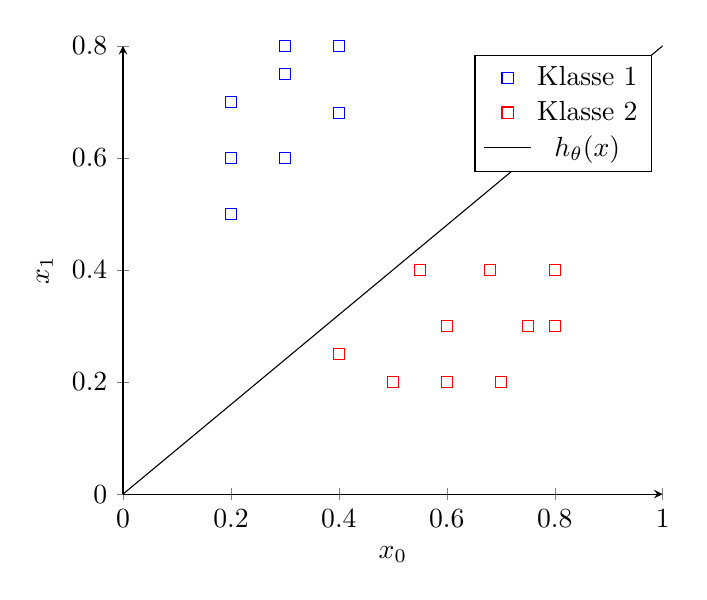
\begin{tikzpicture}
\begin{axis}[
    axis lines = left,
    xlabel = $x_0$,
    ylabel = {$x_1$},
]
\addplot[
    only marks,
    color=blue,
    mark=square,
    ]
    coordinates {
    (0.2,0.7)(0.2,0.5)(0.2,0.6)(0.3,0.8)(0.3,0.6)(0.3,0.75)(0.4,0.8)(0.4,0.68)
    };
\addlegendentry{Klasse 1}
\addplot[
    only marks,
    color=red,
    mark=square,
    ]
    coordinates {
    (0.55,0.4)(0.4,0.25)(0.7,0.2)(0.5,0.2)(0.6,0.2)(0.8,0.3)(0.6,0.3)(0.75,0.3)(0.8,0.4)(0.68,0.4)
    };
\addlegendentry{Klasse 2}
\addplot [
    domain=0:1, 
    samples=100, 
    color=black,
]
{0.8*x};
\addlegendentry{\(h_\theta(x)\)}
\end{axis}
\end{tikzpicture}
\caption{Lineær hypotese skiller datapunktene i to klasser}
\label{figure:separator}
\end{figure}
Separatoren i figur \ref{figure:separator} er en linje i to dimensjoner. En separator i tre dimensjoner vil danne et plan. Å forestille seg en separator i mer enn tre dimensjoner er vanskelig. Heldigvis kan matematikken hjelpe da den ikke bryr seg om våre visuelle begrensninger og fungerer like godt i 128 dimensjoner som i tre. Vi har konkludert med at en lineær modell bør få sjansen til å skille treningseksemplene våre, men hvilken algoritme bør vi benytte? La oss utforske to av de mest brukte og robuste, lineære teknikkene: logistisk regresjon og støttevektormaskiner.\\\\
\subsubsection*{Logistisk regresjon}
I logistisk regresjon modelleres sannsynlighetene som beskriver ulike utfall av en logistisk sigmoid-funksjon(\ref{eq:sigmoid}).
\begin{equation}
g(x) = \frac{1}{1 + e^{-x}}
\label{eq:sigmoid}
\end{equation}
Denne funksjonen tar en hvilken som helst input-verdi og gir en output-verdi i området \([0,1]\). Likning \ref{eq:sigmoid} og figur \ref{figure:sigmoid} representerer den generelle \emph{sigmoid}-funksjonen. Vi ser at ved større positive x-verdier gir funksjonen et resultat nære 1, mens for større negative verdier gir funksjonen et resultat nære 0.
\begin{figure}[h!]
\centering
\begin{tikzpicture}
\begin{axis}[
    axis lines = center,
    xlabel = $x$,
    ylabel = {$y$},
]
\addplot [
    domain=-5:5, 
    samples=100, 
    color=red,
]
{1 / (1 + e^(-x))};
\end{axis}
\end{tikzpicture}
\caption{Ordinær sigmoidfunksjon}
\label{figure:sigmoid}
\end{figure}
La oss si vi har to mulige klasser, \(y \in \{0,1\}\). Hvis \( h_\theta(x) \geq  0.5\), gjetter vi at klassen \(y = 1\). Hvis \( h_\theta(x) < 0.5\), gjetter vi \(y = 0\). Når vi nå kombinerer (\ref{eq:hypotese-kompakt}) og (\ref{eq:sigmoid}) får vi den logistiske hypotesen (\ref{eq:logistic}).
\begin{equation}
h_\theta(x) = \frac{1}{1 + e^{-\theta^{T}x}}
\label{eq:logistic}
\end{equation}
Igjen representerer $\theta$ vektingen av egenskapene $x$ i treningsdataene. 
\begin{equation}
J(\theta) = 
    \frac{1}{m} \sum_{i=1}^{m} cost(h_\theta(x^{(i)}), y)
\label{eq:cost}
\end{equation}
(\ref{eq:cost}) viser formelen for logistisk regresjon. Vi ser at $J(\theta)$ er et gjennomsnitt av en kostnadsfunksjon, definert av hypotesen til hvert treningseksempel og den tilhørende korrekte klassen. 
\begin{equation}
    cost(h_\theta(x^{(i)}), y) = \begin{cases}
    -log(h_\theta(x)), & \text{hvis $y=1$}.\\
    -log(1-h_\theta(x), & \text{hvis $y=0$}.
  \end{cases}
  \label{eq:costdetail}
\end{equation}
Kostnadsfunksjonen (\ref{eq:costdetail}) er definert med delt forskrift slik at kostnaden er 0 dersom klassen er 1 og hypotesen er 1, men dersom klassen er 1 og hypotesen går mot 0, går kostnaden mot uendelig. Den delte forskriften gjør at det samme gjelder for det motsatte tilfellet, der kostnaden er lav dersom klassen er 0 og hypotesen gjetter 0, men øker mot uendelig dersom hypotesen går mot 1.
\begin{equation}
\theta_j \leftarrow \theta_j - \alpha \frac{\delta}{\delta\theta_j}J(\theta)
\label{eq:gradient}
\end{equation}
For å tilpasse $\theta$-verdiene er strategien å minimere kostnadsfunksjonen (\ref{eq:costdetail}). Dette gjøres ved å benytte en oppdateringsregel. Regelen oppdaterer egenskapsvektoren $\theta$ ved å trekke fra resultatet fra den partiellderiverte av kostnadsfunksjonen, dempet av en faktor $\alpha$ (\ref{eq:gradient}). Ettersom den deriverte i et gitt punkt kan sees på som brattheten til kurven i det punktet vil denne oppdateringen tilsvare å stadig ta mindre steg i den retningen som fører mot en lavere verdi. På en to-dimensjonell graf vil det si å følge plottet nedover mot et bunnpunkt, men algoritmen fungerer på samme vis i høyere dimensjoner. Denne oppdateringsregelen kalles \emph{gradient descent} og brukes i flere maskinlæringsalgoritmer for å finne minimumsverdier.

Etter at $\theta$-verdiene er tilpasset av treningsdata kan modellen gjette hvilken klasse et nytt datapunkt tilhører ved å benytte hypotesen (\ref{eq:logistic}). For å lære å skille mellom mer enn to ulike klasser benyttes strategien "en-mot-resten". For hver klasse trenes det en egen hypotese som best mulig skiller mellom denne klassen og alle de andre. Når ny data kommer inn til det trente systemet velges den hypotesen som gir den høyeste sannsynligheten for en viss klassifisering og som dermed er mest sikker på å ha funnet det riktige svaret. I tillegg til å fortelle hvilken klasse dataeksempelet tilhører kan logistisk regresjon fortelle hvor sikker klassifiseringen er. Dette er en god egenskap som støttevektormaskiner mangler.\\

\subsubsection*{Støttevektormaskiner (SVM)}
Støttevektormaskiner er en annen gruppe med maskinlæringsalgoritmer som kan brukes til å løse klassifiseringsproblemer. De er kjent for å være effektive i problemområder med mange dimensjoner og kan oppnå gode resultater selv når antallet datapunkter er høyere enn antallet treningseksempler. De bruker mindre plass i minnet enn andre algoritmer og kan tilpasses til å løse en rekke forskjellige problemer. To ulemper med SVM-er er at de ikke tilbyr direkte estimater på hvor sikker klassifiseringen er og at de, som logistisk regresjon, i utgangspunktet bare kan skille mellom to klasser.

I figur \ref{figure:separator} så vi en lineær hypotese som tydelig delte treningseksemplene i to klasser. Den separerende hypotesen ligger nærmere treningseksemplene for klasse 2. Dette er et resultat av at det er flere treningseksempler av denne typen. Dermed har den lineære metoden produsert en hypotese som ligger nærmere disse treningseksemplene. Vi kan også intuitivt forstå at det må være et uendelig antall forskjellige hypoteser som kan dele datapunktene, men at en hypotese som ligger midt mellom de to klassene av datapunkter vil være den mest robuste. Støttevektormaskiner benytter nettopp denne intuisjonen for å finne en optimal hypotese. Med støttevektormaskiner kalles separatoren et hyperplan som kan danne skiller i flerdimensjonale rom. En optimal deling oppnås av det hyperplanet som har den største avstanden til det nærmeste treningseksempelet hos hver klasse. Denne strategien om å finne den største marginen mellom klassene senker generelt klassifikatorens feilaktighet. Figur \ref{figure:svm} viser et slikt optimalt hyperplan som befinner seg der hvor marginene til hver klasse er maksimal og like stor.
\begin{figure}[h!]
\centering
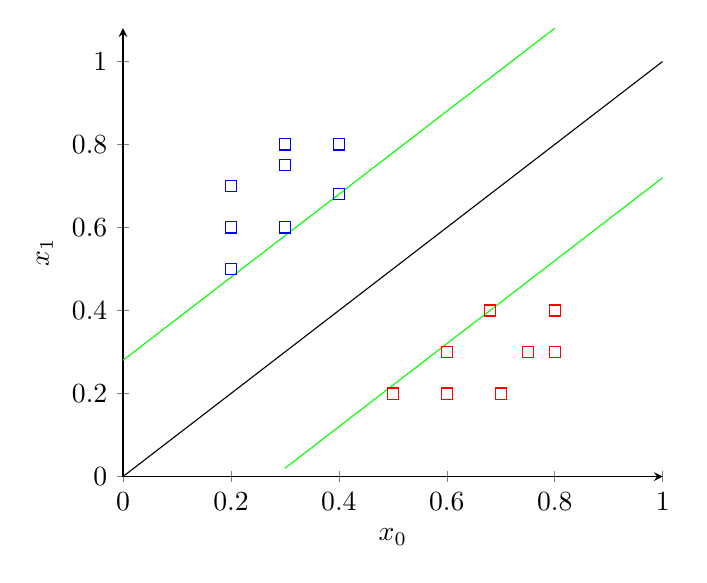
\begin{tikzpicture}
\begin{axis}[
    axis lines = left,
    xlabel = $x_0$,
    ylabel = {$x_1$},
]
\addplot[
    only marks,
    color=blue,
    mark=square,
    ]
    coordinates {
    (0.2,0.7)(0.2,0.5)(0.2,0.6)(0.3,0.8)(0.3,0.6)(0.3,0.75)(0.4,0.8)(0.4,0.68)
    };
\addplot[
    only marks,
    color=red,
    mark=square,
    ]
    coordinates {
    (0.7,0.2)(0.5,0.2)(0.6,0.2)(0.8,0.3)(0.6,0.3)(0.75,0.3)(0.8,0.4)(0.68,0.4)
    };
\addplot [
    domain=0:0.8, 
    samples=100, 
    color=green,
]
{x + 0.28};
\addplot [
    domain=0.3:1, 
    samples=100, 
    color=green,
]
{x - 0.28};
\addplot [
    domain=0:1, 
    samples=100, 
    color=black,
]
{x};
\end{axis}
\end{tikzpicture}
\caption{Det optimale hyperplanet i svart og de to støttevektorene i grønt}
\label{figure:svm}
\end{figure}
Treningen av støttevektormaskiner følger det samme mønsteret som logistisk regresjon, men skiller seg på å ha en annen hypotese og kostnadsfunksjon. Hypotesen er det lineære indreproduktet vi så fra introduksjonen om klassifisering (\ref{eq:hypotese-kompakt}). Kostnadsfunksjonen er enklest forstått gjennom et plot.
\begin{figure}[h!]
\begin{subfigure}{0.5\textwidth}
\centering
\begin{tikzpicture}
\begin{axis}[
    axis lines = center,
    xlabel = $\theta^{T}x$,
    xmin=-2, xmax=2,
    ymin=0, ymax=5,
]
\addplot [
    domain=-2:2, 
    samples=100, 
    color=red,
]
{1 + x};
\addplot [
    domain=-2:-1, 
    samples=100, 
    color=red,
]
{0};
\legend{$cost_0(\theta^{T}x)$}
\end{axis}
\end{tikzpicture}
\end{subfigure}
\begin{subfigure}{0.5\textwidth}
\centering
\begin{tikzpicture}
\begin{axis}[
    axis lines = center,
    xlabel = $\theta^{T}x$,
    xmin=-2, xmax=2,
    ymin=0, ymax=5,
]
%\addlegendentry{$cost_0(\theta^{T}x)$}
\addplot [
    domain=-2:2, 
    samples=100, 
    color=blue,
]
{1 - x};
\addplot [
    domain=1:2, 
    samples=100, 
    color=blue,
]
{0};
\legend{$cost_1(\theta^{T}x)$}
\end{axis}
\end{tikzpicture}
\end{subfigure}
\caption{Støttevektormaskinens kostnadsfunksjoner}
\label{figure:svmcost}
\end{figure}
(\ref{figure:svmcost}) viser de to kostnadsfunksjonene. Dersom klassen $y=1$ ønsker vi at hypotesen $\theta^{T}x \geq 1$. Dersom klassen $y=0$ ønsker vi at hypotesen $\theta^{T}x \leq -1$

Treningen består dermed igjen av å minimere (\ref{eq:svmcost}) med den samme oppdateringsregelen som for logistisk regresjon (\ref{eq:gradient}), men med en ekstra, justerbar parameter $C$ som avgjør hvor mye man ønsker å unngå å feilklassifiere hvert treningseksempel. Med en stor $C$-verdi vil optimaliseringen velge et hyperplan med mindre marginer, dersom dette hyperplanet gjør en bedre jobb på å få alle treningsdataene klassifisert riktig. En lav $C$-verdi lar optimaliseringen finne et hyperplan med større marginer, selv dersom dette hyperplanet feilklassifiserer flere treningseksempler.
\begin{equation}
J(\theta) = 
    C \sum_{i=1}^{m} y^{(i)}cost_1(h_\theta(x^{(i)})) + (1-y^{(i)})cost_0(h_\theta(x^{(i)}))
\label{eq:svmcost}
\end{equation}
Den typen SVM vi har presentert her er en såkalt lineær SVM eller en SVM uten kjerne. Ved å benytte et såkalt \emph{kernel trick} kan SVM-er også modellere ikke-lineære funksjoner. Dette gjør SVM-er svært fleksible til å håndtere ulike data. I dette prosjekt er vi kun interessert i de lineære modellene. For å håndtere klassifisering av flere klasser benyttes gjerne den samme "en-mot-resten"-strategien som i logistisk regresjon. Denne ender altså opp med å trene $n$ klassemodeller og modellen med det beste resultatet benyttes.\\

\subsection{Brukergrensesnitt}
\citet{victor06} påpeker at programvare eksisterer for å hjelpe folk med tre ting: å lære, å skape eller å kommunisere.
\begin{itemize}
\item \emph{Informasjonsprogramvare} hjelper folk med å lære. Vi bruker informasjonsprogramvare for å konstruere og manipulere en intern representasjon av informasjonen.
\item \emph{Manipulasjonsprogramvare} hjelper folk med å skape. Vi bruker manipulasjonsprogramvare for å skape og manipulere en virtuell modell, representert i datamaskinen. Denne typen programvare kan bli forstått som et virtuelt verktøy, som en malingskost eller skrivemaskin, som benyttes som et grensesnitt mellom skaperen og sluttproduktet.
\item \emph{Kommunikasjonsprogramvare} hjelper oss med å kommunisere. Vi bruker kommunikasjonsprogramvare for å skape og manipulere en intern modell som er delt, forstått og synkronisert mellom flere mennesker. Kommunikasjon kan sees på som å lage et svar på tillært informasjon. Den eksterne modellen en bruker kommuniserer, er den interne modellen brukeren har lært.
\end{itemize}
Brukere i smarte hjem trenger programvare til å gi kommandoer til hjemmet, som å skru på lyset i et rom eller låse utgangsdøra. De trenger også programvare for å lære om hjemmets tilstand, som å se temperatur, status på oppvaskmaskina eller om det mangler matvarer i kjøleskapet. For å lære om hjemmet bør det designes informasjonsprogramvare. For å gi kommandoer til hjemmet passer kommunikasjonsprogramvare best. Hvordan kan relevant informasjon om hjemmet kan presenteres for brukeren? Hvordan kan man effektivt og naturlig kan gi kommandoer til hjemmet? 

I introduksjonen definerte jeg IUI til å være grensesnitt mellom mennesker og datamaskiner med et mål om å være mer effektive og mer naturlige i bruk, enn tradisjonelle grensesnitt. \citet{Kaufmann98} påpeker at dette oppnås gjennom å representere, resonnere og handle på modeller av brukeren, domenet, oppgaven, diskusjonen og mediumet. IUI er en del av HCI, ergonomikk, kognitiv vitenskap og AI. Målet til HCI er å gjøre datamaskiner mer hjelpsomme og enklere å bruke. \citet{Lieberman09} skriver om hvordan HCI og AI er relaterte og hvordan de bør samarbeide og kan lære av hverandre for å løse målene våre. Det må inses at det er \emph{trade-offs} mellom systemets pålitelighet og grad av konsekvens, og systemets evne til å forstå hva brukeren ønsker og å tilby hjelp. Lieberman påpeker videre at avanserte brukergrensesnitt muligens trenger \emph{tutorials} for å gjøre brukerne komfortable med systemet. Brukerens behov forandrer seg stadig så å ta utgangspunkt i et dynamisk system gir fleksibilitet til å håndtere framtidige forandringer. HCI har investert mye i forskning på modeller som \emph{GOMS} eller \emph{key-stroke}, for å modellere sammenhengene mellom oppgaver, og operasjonene som trengs for å fullføre dem i et gitt grensesnitt. Disse modellene hjelper med å evaluere effektiviteten i brukergrensesnittene. Å introdusere intelligens i systemene kan la brukere unngå utførelsen av en rekke operasjoner for å nå et mål. Brukeren kan i stedet angi et overordnet mål og det er så opp til systemet å finne ut hva som må gjøres for å oppnå målet.\\

\subsubsection*{Smarttelefoner og andre touch-skjermer}
Touchskjermer i form av smarttelefoner og nettbrett er nå vidspredte og populære. Det er en interaksjonsform folk bør være komfortable med å bruke i det smarte hjemmet. At nesten alle har smarttelefoner med seg til enhver tid gjør også at muligheten til informasjon om og styring av hjemmet alltid er tilgjengelig.

\citet{koskela04} undersøkte forskjellige brukergrensesnitt for å styre smarte hjem. De evaluerte bruken av en pc, en tv med fjernkontroll og en mobiltelefon. Resultatene viste at en pc fungerte best som en sentral enhet for å kontrollere aktiviteter som kan planlegges eller bestemmes på forhånd. Dette gjaldt å sette opp automatiseringer, slik som at gardinene skal trekkes for og at lysene skrus på til et visst tidspunkt. Mobiltelefonen ble funnet til å være det beste alternativet for direkte kontroll. Denne studien ble gjort i 2004 og resultatene kan derfor antas å være noe daterte, men resultatet om at en bærbar, mobil enhet var det beste for å direkte kontrollere omgivelsene er nyttig. Dagens smarttelefoner er kapable til langt mer enn mobiltelefonen fra 2004. Det virker derfor rimelig å konkludere med at bærbare touch-skjermer er et godt alternativ for å tilby interaksjon med hjemmet.\\

\subsubsection*{Omgivelsesskjermer}
I kapitellet om smarte hjem nevnte jeg AmI og teknologi overalt i miljøet. En teknologi det forskes på i AmI er omgivende skjermer. Informasjonskilder, andre mennesker og omgivelsene skal kunne sees og interageres med når det er behov for det. Å ha informasjonskilder tilgjengelig forskjellige steder i hjemmeomgivelsene kan gi nye muligheter for samarbeid mellom mennesker i aktiviteter som omhandler både lek og arbeid.

Forskjellige interaksjonssoner beskrives av \citet{streitz05}. De omtaler interaksjonssonene omgivende, notifikasjon og interaksjon. Avhengig av hvilken sone en bruker befinner seg i vil omgivelsesskjermen regulere hvordan informasjonen og interaksjonsmetoden presenteres. \emph{Proxemics} foreslås av \citet{greenberg11} som en tilnærming for å gi enheter en mer naturlig oppførsel. De stipulerer at brukere naturlig forventer at når enhetene deres nærmer seg andre enheter eller gjenstander i omgivelsene, øker tilkoblingen og interaksjonsmulighetene forbedres. Bruken av soner gir mulighet til å tilby forskjellige visninger og interaksjoner basert på forskjellige dimensjoner. Greenberg et al. omtaler fem målbare dimensjoner av proxemics: \emph{avstanden} mellom enheter og brukere, \emph{retning} gir et mål på vinkelen mellom enheter og brukere\footnote{Det finnes allerede enheter som gjør bruk av retning, for eksempel ved å skru seg av når folk ikke ser på dem.}, \emph{bevegelse} omfatter forandring i distanse over tid, \emph{identitet} beskriver en enhet i et gitt detaljnivå og \emph{plassering} beskriver posisjonen til enheten. Proxemics kan i sin helhet være med på å tilby en mer naturlig interaksjon med enhetene våre og kan kanskje være det neste steget for utviklingen av interaksjonsapplikasjoner.\\

\subsubsection*{Gester}
Interaksjon gjennom gester er et forsøk på å tilby en mer naturlig interaksjon med datamaskinen. Kroppsspråket er tross alt en stor del av mellommenneskelig kommunikasjon, så hvorfor ikke forsøke å utvide det til kommunikasjon mellom menneske og maskin. De fleste prosjektene som utforsker bruker av gester benytter kameraer som måler farger og dybde, samt avanserte datasynsalgoritmer for å gjøre mening av dataene. Sammen kan disse prosessere informasjonen og danne grunnlaget for et system som kan gjenkjenne kompliserte gester. Et eksempel omtales av \citet{homeos}, der \emph{Kinect}-kameraet\footnote{\url{https://www.microsoft.com/en-us/kinectforwindows/develop/}} ble brukt til å forstå gester.

\citet{96bytes} hos Microsoft Research har utviklet en keyboard-prototype som forstår enkle gester. Prototypen forsøker å danne en bro mellom touch-grensesnitt og tradisjonelle keyboard. Keyboardet har 64 sensorer parvis plassert mellom tastene, der 32 sender et IR-signal og de andre 32 sanser reflekterte signaler. Av disse dataene dannes det tre bilder: et av rådataene, et som viser historie over nærhet og et med historie over bevegelse. Prosjektet brukte \emph{random forests} for å klassifisere gestene. Bruksområdet for keyboardet er å bevege seg mellom applikasjoner, zoome eller scrolle, uten å måtte ta hendene vekk fra keyboardet.\\

\subsubsection*{Multimodalitet}
Multimodale brukergrensesnitt analyserer og forstår flere kommunikasjonskanaler samtidig. Dette kan gi systemer som er mer naturlige å interagere med. For eksempel kan mennesker kommunisere med datamaskinen gjennom tale og kroppsspråk. Å tilby flere kommunikasjonskanaler til brukeren kan gjøre systemet mer robust, ved å kombinere delvis informasjon fra flere kilder. Multimodalitet kan også gi brukeren muligheten til å selv velge den foretrukne modaliteten. Etter at inputsignalene har nådd systemet må disse analyseres og forstås. Dette steget kalles \emph{fusion}, og omhandler integrasjonen av modalitetene. Det finnes ulike detaljnivåer å integrere signalene på. Et høyere semantisk nivå av fusion er når signalene først forstås hver for seg, og deretter integreres. Alternativt kan datastrømmene integreres tidlig, før de forstås. \citet{dumas09} omtaler de ulike formene for fusion som \emph{data-level}, \emph{feature-level} og \emph{decision-level} \citet{jaimes07} kaller de samme kategoriene \emph{early}, \emph{intermediate} og \emph{late fusion techniques}. Late/decision-level fusion er den mest brukte teknikken. Den involverer ofte uavhengige klassifikatorer for hver inputstrøm. Deretter kombineres disse videre til en enkelt, felles klassifikator. Ettersom kildene datastrømmene håndteres uavhengig trenger de ikke å utføres samtidig. Et multimodalt system kan også ha flere modaliteter for å gi feedback. \emph{Fission} er når systemet avgjør hvilke modaliteter som skal benyttes for å kommunisere tilbake til brukeren.\\

\subsubsection*{Hjerne-maskin-grensesnitt}
Hjerne-maskin-grensesnitt (BCI) er teknologi for å la hjernen kommunisere direkte med maskinen. Forskningen rundt denne teknologien dreier seg hovedsaklig om å hjelpe eller forbedre funksjonshemmede mennesker. Mennesker med motorkontrollen i orden bruker kroppen sin som et grensesnitt til verden. Dette systemet har utviklet seg over millioner av år og fungerer utmerket. Brukergrensesnitt til datamaskiner er et helt nytt konsept. Dersom det er problemer mellom kroppene våre og datamaskiner, ville det ikke vært mest naturlig å sette spørsmål ved datamaskinen, ikke kroppen? Datamaskinene bør vel tilpasses til å best mulig bruke våre kropper, i stedet for å forbigå kroppen totalt. Vi er allerede i ferd med å miste kroppene våre. Vi sitter stille mesteparten av dagen, både gjennom arbeid, reise og fritid. Dette er teknologi som er verdt å utforske for å hjelpe funksjonshemmede. Det er også interessant å se hva datamaskinene kan lære om følelsene våre ved å lytte på hjerneaktiviteten. Men jeg er usikker på om BCI er verdifullt å utforske og om det er det vi ønsker for framtidens friske mennesker.

\subsubsection*{Dynamiske brukergrensesnitt}
I kapittel \ref{ch:smartehjem} så vi på hva brukerene ønsker seg. Noen av disse ønskene kan være vanskelig å implementere uten å bryte noen av de andre ønskene. For eksempel som at systemet skal forstå konteksten i omgivelsene, uten å være påtrengende og oppleves som overvåkende. Det viktigste for de spurte gruppene var å selv være i kontroll av et system som var enkelt å bruke og som ga muligheter til å styre huset, inkludert elektriske apparater, hvitevarer, hjemmeunderholdning, lys og varme. Det er kanskje viktigere for vanlige brukere at det tilbys gode styringsmuligheter, enn at systemet er proaktivt og forsøker å forstå hva brukeren ønsker?

\citet{directmanipulation} diskuterer om direkte manipulasjon er det beste, eller om brukergrensesnitt skal tilpasse seg dynamisk og forsøke å hjelpe brukeren. Schneiderman argumenterer for at vi bør utnytte øyets formidable kapasitet og anvende langt \emph{flere} ikoner, knapper og vinduer enn det som er vanlig i dag. 4000 eller flere elementer på skjermen gir brukeren en full oversikt over mulige valg. Oversikt er det viktigste. Brukeren kan deretter zoome inn på det de er ute etter og filtrere ut det de ikke er interessert i. Dette gir brukeren en følelse av kontroll og dermed en ansvarsfølelse til avgjørelsene de tar. Maes argumenterer for verdien av programvareagenter; programvare som kan ta egne avgjørelser. Grunnlaget for å ønske dette er datamaskinmiljøer som øker i kompleksitet og en brukermasse som øker i naivitet. Når det blir for mye å holde styr på må oppgaver delegeres og programvareagenter kan da være til hjelp. Vi trenger "ekstra øyne" til å finne informasjon vi kan være interessert i. Et eksempel på en slik agent er anbefalingssystemer, som når \emph{Netflix} anbefaler filmer basert på hva brukeren og andre liknende brukere har sett på\footnote{\url{https://www.netflix.com/no/}}. Eller \emph{Amazon}, som foreslår varer basert på hva andre brukere som kjøpte den samme varen også viste interesse i. Det kan være stor verdi i at systemet foreslår ting brukeren aldri ville tenkt på eller kommet borti\footnote{\url{http://www.amazon.com/}}. Maes er enig i at det trengs godt designede grensesnitt for manipulasjon, men at det er en rekke oppgaver brukeren ikke har lyst til å utføre og at programvareagenter kan ta seg av disse oppgavene.

\citet{rogers06} påpeker at forskningsmiljøet har møtt problemer med å forstå den store variasjonen i hva folk gjør, hvilke motiver de har, når de gjør det og hvordan de gjør det. Konteksten rundt folks dagligdagse liv er svært subtil. Dette gjør det vanskelig, om ikke umulig, å implementere kontekst slik at det kan gjøres nyttige spådommer om hva mennesker føler, hva de ønsker, eller hva de trenger, i et gitt øyeblikk. Hun argumenterer for et skifte fra proaktiv databehandling til proaktiv mennesker. Allestedsnærværende teknologier bør designes slik at brukere kan interagere med dem mer aktivt. Mennesker, i stedet for maskiner, bør ta initiativet til å være konstruktive, kreative og engasjere i interaksjoner. I stedet for å pakke omgivelsene med all slags forsvinnende teknologi, bør vi tenke på teknologien som et sett med verktøy og overflater, som er mobile og tilrettelegger for samarbeid. Informasjonskilder, andre mennesker og omgivelsene kan sees og interageres med når det er behov for det. Vi må få tilbake gleden med interaksjon på innovative måter.

Interaktiv media gir brukere personlig tilgang til informasjon. \citet{ishizaki96} presenterer \emph{maDes}, en arkitektur som oppfordrer designere til å anse et \emph{designproblem} som en kontinuerlig strøm, framfor en samling diskret problemer, og en \emph{designløsning} som en entitet generert av den dynamiske aktiviteten til \emph{designelementer}, framfor et sett med designelementer med faste attributter. \emph{maDes} modellerer en designløsning som et system bestående av en samling av mindre designsystemer. Hvert system er en \emph{designagent} og er ansvarlig for å presentere en bestemt type informasjon. En designagent kan tilpasse hvordan informasjon vises ut fra forandring i kontekst og gjennom samarbeidet med andre designagenter. I designet av programvare-basert media opplever designeren at det er umulig å designe en løsning til et spesifikt problem og at han i stedet må representere en måte å designe programvare på som kan generere løsninger mens programmet kjører.\\ 

\subsubsection*{Tale}
\label{ch:tale}
Å gi datamaskinen evnen til å forstå og utøve tale er en av teknikkene fra AI som har hatt kommersiell suksess. Talegjenkjenning benyttes daglig av brukere verden over for å gi navigasjonsinstrukser til bilene sine, gjøre søk på nettet eller å skrive gjennom diksjon. Tale er en attraktivt interaksjonsform i alle tilfeller der brukeren kan ha bruk for å gjøre andre ting med hendene, eller der han ikke har muligheten til å bruke dem. Det er ingen enkel oppgave å gjenkjenne tale. Lydene brukeren lager inneholder ofte støy og det finnes en rekke setninger som høres like ut når de sies fort. Når vi skriver setninger er det mellomrom mellom ordene, men i tale er det setninger som uttales uten pause mellom ordene. Det er også mange ord som uttales likt, men skrives forskjellig og har forskjellig betydning avhengig av kontekst. Carnegie Mellon University påpeker at virkeligheten med tale ikke er så enkelt som man skulle tro. Intuisjonen er at tale er bygget opp av ord, og at hvert ord består av fonemer. I virkeligheten er det desverre svært annerledes. Tale er en dynamisk prosess uten klare skiller mellom ulike deler. De moderne måtene å beskrive tale på er i større eller mindre grad basert på sannsynligheter. Denne måten å se situasjonen på lar oss forstå at talegjenkjenning aldri vil være 100\% korrekt\footnote{\url{http://cmusphinx.sourceforge.net/wiki/tutorialconcepts}}. Den vanlige måten å gjenkjenne tale på er følgende: man mottar en bølgeform, splitter den inn i ytringer delt av stillhet og forsøker så å gjenkjenne hva som blir sagt i hver ytring. For å gjøre dette tar vi alle mulige kombinasjoner av ord og forsøker å matche dem med lyden. Vi velger så den kombinasjonen som passer best.

Tre modeller benyttes i talegjenkjenning for å matche ord med lyd. En akustisk modell, en ordbok og en språkmodell. Den akustiske modellen holder akustiske egenskaper for kombinasjoner av fonemer. En enkel fonetisk ordbok knytter ord med fonemer. Denne naive varianten er ikke veldig effektiv ettersom den ikke tar større hensyn til forskjellige uttaler, men den fungerer som regel i praksis. Maskinlæring kan benyttes her for å lære langt mer nyanserte sammenhenger. En språkmodell brukes for å innsnevre søket etter det passende ordet. Den definerer hvilke ord som kan følge etter det foregående gjenkjente ordet og hjelper dermed med å fjerne ord som ikke er sannsynlige. For å oppnå en god presisjon må språkmodellen utføre en god jobb på å begrense søkeområdet for mulige ord. Den må altså være svært god på å gjette det neste ordet. En språkmodell kan for eksempel si at setningen "Skru av lyset" er 1000 ganger så sannsynlig som "Skru av fryse". \citet{russellnorvig10} omtaler talegjenkjenning som å være identifikasjonen av en sekvens av ord ut i fra et akustisk signal. Talegjenkjenning handler om å finne den mest sannsynlige sekvensen av ord. De fleste talegjenkjenningssystemene i dag benytter en språkmodell etter \emph{Markov-antakelsen}. Dette betyr at det nåværende ordet kun avhenger av et visst antall foregående tilstander. Det nåværende ordet representeres gjerne som en enkelt, tilfeldig variabel. Dette gjør modellen i sin helhet til en \emph{Hidden Markov Model (HMM)}. Modellen beskriver en sekvens av tilstander der overgangen er gitt av en sannsynlighet. Det er en generell modell som kan beskrive alle sekvensielle prosesser og den har vist seg å være spesielt praktisk for å dekode tale. 
